\documentclass[a4paper,12pt]{article}
\usepackage[backend=biber,sorting=none,style=gost-numeric,autolang=other]{biblatex} % библиография
\usepackage{mathtext} %русские буквы в формулах
\usepackage[T2A]{fontenc}
\usepackage[utf8]{inputenc}
\usepackage[english,russian]{babel}
\usepackage{amsmath}
\usepackage{fancyvrb}
\usepackage{formular}
\usepackage{setspace} % управление междустрочными интервалами
%поля документа
\usepackage[left=3cm,right=1cm,top=2cm,bottom=2cm]{geometry}

\usepackage{misccorr} % точки в конце номеров разделов, использовать перед пакетом ccaption!
\usepackage{ccaption} % изменения подписей к рисункам и табл.

\usepackage[nooneline]{caption} 
\captionsetup[table]{justification=raggedright} % заголовок таблицы выравнивается влево
\captionsetup[figure]{justification=centering,labelsep=endash} % заголовок рисунка - по центру
% отступ перед первым абзацем
\usepackage{indentfirst}
%вставка изображений
\usepackage{graphicx}
% счетчики
\usepackage{totcount}
% управление содержанием
\usepackage{tocloft}
\usepackage[english,russian]{babel}
% управление таблицами и рисунками
\usepackage{float}
% управление системами
\usepackage{cases}
\newcounter{mycitecount}                                %% Счётчик библиографии
\AtEveryBibitem{\stepcounter{mycitecount}}              %% Работает для biblatex

\usepackage[figure,      %
            table,       %
            mycitecount, xspace ]{totalcount}           %% Подсчёт общего количества объектов в документе

% окружение для листингов - с нумерацией строк слева
\DefineVerbatimEnvironment{MyCode}{Verbatim}{frame=lines,numbers=left,numberblanklines=false,framesep=5mm}

% автоматическая нумерация листингов
\newfloat{Program}{phb}{lop}
\floatname{Program}{Листинг}
\floatstyle{ruled}

\setcounter{secnumdepth}{3} % глубина нумерации до подразделов

%если нужны точки в оглавлении для разделов - раскомментируйте следующую команду
%\renewcommand{\cftsecleader}{\cftdotfill{\cftdotsep}}

\addto\captionsrussian{%
\renewcommand{\figurename}{Рисунок}%
\renewcommand{\tablename}{Таблица}%
}

% дефис в подписи к рисункам
\captiondelim{ -- } 

% Настройки для окружений с подчеркиваниями для подписей и пр.
\setFRMfontencoding{T2A}
\setFRMdfontencoding{T2A}
% thanks to A.Starikov
\setFRMfontfamily{cmr}
\setFRMdfontfamily{ptm}
\setFRMdfontsize{10pt}

% задает длину поля для подписи на титульной странице
\newFRMfield{xtitlesign}{32mm}

% поле для факультета или кафедры
\newFRMfield{fcath}{65mm}

%имя файла с библиографией в формате BibTex
\addbibresource{rbiblio.bib}

\begin{document}

% счетчики страниц, рисунков, таблиц
\regtotcounter{page}
\regtotcounter{figure}
\regtotcounter{table}

\renewcommand{\refname}{\centerline{СПИСОК ИСПОЛЬЗОВАННОЙ ЛИТЕРАТУРЫ}} 
\renewcommand{\contentsname}{\centerline{СОДЕРЖАНИЕ}} 
%\renewcommand{\refname}{Список источников}  % По умолчанию "Список литературы" (article)
%\renewcommand{\bibname}{Литература}  % По умолчанию "Литература" (book и report)

% титульная страница
\thispagestyle{empty}
\begin{center} \small
\textbf{МИНИСТЕРСТВО НАУКИ И ВЫСШЕГО ОБРАЗОВАНИЯ РОССИЙСКОЙ ФЕДЕРАЦИИ}\\
ФЕДЕРАЛЬНОЕ ГОСУДАРСТВЕННОЕ АВТОНОМНОЕ ОБРАЗОВАТЕЛЬНОЕ УЧРЕЖДЕНИЕ
ВЫСШЕГО  ОБРАЗОВАНИЯ\\
«Национальный исследовательский ядерный университет «МИФИ»\\
\textbf{Обнинский институт атомной энергетики} – \\
филиал федерального государственного автономного образовательного учреждения высшего\\
образования «Национальный исследовательский ядерный университет «МИФИ»\\
(ИАТЭ НИЯУ МИФИ)
\end{center}
%\vfill
\medskip

\begin{center}
\begin{tabular}{rl}
Отделение & \useFRMfield{fcath}[\large Интеллектуальные кибернетические системы] \\ 
Направление подготовки & \useFRMfield{fcath}[\large Информационные системы и технологии] \\ 
\end{tabular} 
\end{center}

\vfill

\large 

\begin{center}
	Научно-исследовательская работа \\
	
	\medskip
	
	\textbf{\Large 
		Разработка наземной системы позиционирования и навигации микродрона с применением компьютерного зрения
	}
	
\end{center}

\vspace{1cm}

\begin{tabular*}{\textwidth}{lcr}
Студент группы ИС-Б17 & \useFRMfield{xtitlesign} & В. Ю. Петренко\\
& & \\
Руководитель & & \\
к.т.н., доцент каф. ИС & \useFRMfield{xtitlesign} & О. А. Мирзеабасов\\
& & \\
Научный консультант & & \\
Инженер ЦОНД & \useFRMfield{xtitlesign} & М. И. Турицын\\
& & \\
\end{tabular*}


\vfill
\large

\begin{center}
Обнинск, 2020 г
\end{center}

\onehalfspacing

\pagebreak

% реферат
\thispagestyle{empty}

\section*{\centering РЕФЕРАТ}
% объем не больше страницы, подобие аннотации
% возможно, кол-во источников придется вставлять вручную
\total{page} стр., \total{table} табл., \total{figure} рис. , \totalmycitecounts ист. 

% КЛЮЧЕВЫЕ СЛОВА В ВЕРХНЕМ РЕГИСТРЕ
БПЛА, КВАДРОКОПТЕР, РОБОТОТЕХНИКА, КОМПЬЮТЕРНОЕ ЗРЕНИЕ, АВТОНОМНЫЙ ПОЛЕТ, НАЗЕМНАЯ СТАНЦИЯ

Работа посвящена разработке экспериментального образца наземной станции и микродрона, а также выбору их протокола общения.
Суть работы заключается в модификации и доработке существующих робототехнических решений на основе БПЛА посредством выноса бортового компьютера в наземную станцию, благодаря чему станет возможно уменьшение размеров и стоимости квадрокоптера.
Наземная станция представляет собой совокупность компьютера и радиомодулей для получения и последующей обработки изображения с квадрокоптера. Результаты обработки отправляются по радио на борт квадрокоптера в виде управляющих сигналов.
Таким образом, квадрокоптер получает дополнительную систему координат без использования датчиков подобных GPS, а также возможность навигации с использованием компьютерного зрения.
% определяет свое место в пространстве 

Разработанный ПАК дает возможность создать образовательный робототехнический комплект на основе беспилотника. Вынося бортовой компьютер в наземную станцию, получаем такие преимущества, как безопасность, низкая стоимость, в том числе существенно удешевляется ремонт.
% простота эксплуатации
\pagebreak
\thispagestyle{empty}

\section*{\centering ОПРЕДЕЛЕНИЯ}

Квадрокоптер --- БПЛА мультироторного типа с четырьмя несущими винтами

UART -- universal asynchronous receiver/transmitter, аппаратный последовательный интерфейс


\pagebreak

\section*{\centering ОБОЗНАЧЕНИЯ И СОКРАЩЕНИЯ}

НИР --- Научно-исследовательская работа

БПЛА --- Беспилотный летательный аппарат

ПАК --- Программно-аппаратный комплекс

MAVLink -- Micro Air Vehicle Link

FPV -- First Person View

ВМГ -- Винто-моторная группа

UART -- Universal asynchronous receiver/transmitter, аппаратный последовательный двусторонний интерфейс для подключения периферии

%HITL -- hardware in the loop, программная симуляция аппарата
%SITL -- software in the loop, ПО для воссоздания поведения системы реального времени в симуляции
Бод-рейт -- скорость передачи данных через UART
\pagebreak

\tableofcontents

\pagebreak

\section*{\centering ВВЕДЕНИЕ}
\addcontentsline{toc}{section}{ВВЕДЕНИЕ}
Сфера беспилотных и робототехнических систем растет с неимоверной скоростью -- в 2020 году их количество увеличилось вдвое по сравнению с прошлым годом. На рынке труда спрос на специалистов данной области не удовлетворен и только растет. В связи с чем в программу основного общего образования включают курсы программирования и робототехники, закупаются образовательные комплекты на основе квадрокоптеров. \cite{minobr}

Однако комплектов, способных удовлетворить спрос образовательных учреждений, не так много, самыми известными являются Геоскан Пионер, COEX Клевер и NanoPix MiniBot.

Первые два комплекта представляют собой квадрокоптеры диаметром до 300мм с микрокомпьютером на борту, выполняющим все вычислительные операции. Падения таких беспилотников приводят к риску для окружающих, а так же дополнительным тратам, так как ломается дорогостоящее оборудование. Из-за больших размеров возникает потребность в большом помещении, огражденном сеткой. Для Пионера также необходимы дополнительные датчики для его позиционирования, которые необходимо размещать в углах помещения. Эти устройства не входят в комплект и их стоимость близка к стоимости самого квадрокоптера.

NanoPix MiniBot -- миниатюрный комплект, безопасный для окружающих, однако не обладает бортовым компьютером, а на малых вычислительных мощностях не способен выполнять сложные задачи и автономные миссии.

В ходе эксплуатации комплекта Клевер в рамках участия на соревнованиях WorldSkills Russia "Молодые профессионалы" появилась идея как усовершенствовать/модиф сущ комплекты
 
 вывести борт комп в наземную станцию
 все вышеперечисл факторы обусловлен тем что квад должен иметь  борт пк=увел размер и все вытек последств
 и потом первое предло
 
 таким образом суть что будет передаваться сигнал с наземки
 
Идея состоит в том, чтобы вынести квадрокоптера микрокомпьютер, тем самым уменьшив размеры дрона и возможные риски.

когда на борту-ламаеца

Таким образом, получается программно -- аппаратный комплекс из микроквадрокоптера и наземной управляющей станции.
Цель данной научно -- исследовательской работы разработать аппаратную часть такого комплекта, а также описать протоколы взаимодействия наземной станции с квадрокоптером.
 % текст введения в файле intro.tex
\pagebreak
\pagebreak
% первая часть

\section{Предметная область}

\subsection{что-то}
о чем-то
https://www.genebm.com/drone-bytes/software-design/middlewares-ros-fprime часть обоснования выбора рос

\subsection{Математическая модель квадрокоптера}
Рассмотрим квадрокоптер с известными физическими параметрами, движением которого можно управлять, изменяя скорости вращения винтов. Для формального описания динамики движения квадрокоптера как твердого объекта в трёхмерном пространстве необходимо ввести в рассмотрение две системы координат (СК):
1. Неподвижную систему координат (НСК), в качестве которой выступает нормальная земная система координат с заданными перпендикулярными друг другу координатными осями \(O_{g}X_{g}\), \(O_{g}Y_{g}\), и \(O_{g}Z_{g}\), причем ось \(O_{g}Z_{g}\) направлена противоположно вектору силы тяжести.
2. Связанную с квадрокоптером систему координат (ССК), центр которой размещен в центре масс аппарата, а оси OX, OY, и OZ параллельны и сонаправлены с осями неподвижной системы. Угловое положение аппарата зададим тремя углами Эйлера: углами крена \(\phi\), тангажа \(\theta\) и рыскания \(\psi]\), определяющими вращение вокруг осей OX, OY, и OZ соответственно. Основываясь на ранее рассмотренных системах координат можно утверждать о том, что квадрокоптер имеет шесть степеней свободы, а именно три линейных координаты [x; y; z ] и три угловых \([\theta, \phi, \psi]\). В качестве управляющих каналов выступают скорости вращения роторов (рис. 1), которые создают динамику движения БПЛА в пространстве. Согласно [1–3], возникающие в результате подачи управляющих воздействий силы и моменты пропорциональны квадрату угловых скоростей винтов \(\Omega^2\) . Поэтому, для достижения желаемого режима работы БПЛА, необходимо связать совокупность управляющих воздействий со степенями свободы БПЛА, через уравнения связи, которые определяют основные режимы движения квадрокоптера в пространстве.

% ~\ref{fig:ris1}
\begin{figure}[H]
	\centering
	\includegraphics[width=0.5\linewidth]{pics/ris1}
	\caption{Связанная система координат квадрокоптера
	}
	\label{fig:ris1} % эта метка позволяет ссылаться на рисунок в тексте
\end{figure}
В качестве первого режима БПЛА \(U_{1}\) рассмотрим движение вдоль оси OZ, принадлежащей ССК. Данное движение обеспечивается одновременным увеличением скоростей винтов на одинаковое значение угловой скорости \(\Delta a\). Полученное при этом движение (рис. ~\ref{fig:ris1}) характеризуется взлетом или посадкой квадрокоптера (при нулевых значениях тангажа и крена) и описывается следующим выражением:
\begin{equation}
U_{1}=b(\Omega_{1}^2+\Omega_{2}^2+\Omega_{3}^2+\Omega_{4}^2)
\end{equation}
где b – аэродинамическая составляющая тяги винта.
В качестве второго режима движения БПЛА \(U_{2}\) необходимо взять поворот вокруг оси OX, принадлежащей ССК. Данное движение достигается путем увеличения/уменьшения на величину \(\Delta a\) значения \(\Omega_{4}\) левого винта и уменьшением/увеличением на величину \(\Delta b\) значения \(\Omega_{1}\)
правого. Полученное при этом движение характеризуется изменением угла крена \(\phi\) (рис. ~\ref{fig:ris2}) и описывается следующим выражением:
\begin{equation}
U_{2}=lb(-\Omega_{2}^2-\Omega_{4}^2)
\end{equation}
где l – расстояние между центром квадрокоптера и центром винта.
% ~\ref{fig:ris2}
\begin{figure}[H]
	\centering
	\includegraphics[width=0.5\linewidth]{pics/ris2}
	\caption{Вращение квадрокоптера вокруг оси OX
	}
	\label{fig:ris2} % эта метка позволяет ссылаться на рисунок в тексте
\end{figure}
В качестве третьего режима движения \(U_{3}\) необходимо взять поворот БПЛА вокруг оси OY , принадлежащей ССК. Данное движение достигается путем уменьшения/увеличения на величину \(\Delta a\) значения \(\Omega_{1}\) фронтального винта и увеличения/уменьшения на величину \(\Delta b\) значения \(\Omega_{3}\) заднего. Полученное при этом движение характеризуется изменением угла тангажа \(\theta\) (рис. ~\ref{fig:ris2}, а) и описывается следующим выражением:
\begin{equation}
U_{3}=lb(-\Omega_{1}^2-\Omega_{3}^2)
\end{equation}
% ~\ref{fig:ris3}
\begin{figure}[H]
	\centering
	\includegraphics[width=0.5\linewidth]{pics/ris3}
	\caption{Вращение вокруг оси OY
	}
	\label{fig:ris3} % эта метка позволяет ссылаться на рисунок в тексте
\end{figure}
% ~\ref{fig:ris4}
\begin{figure}[H]
	\centering
	\includegraphics[width=0.5\linewidth]{pics/ris4}
	\caption{Вращение вокруг оси OZ
	}
	\label{fig:ris4} % эта метка позволяет ссылаться на рисунок в тексте
\end{figure}
Рис. 3 – Режимы движения квадрокоптера

В качестве последнего, четвертого, режима движения \(U_{4}\) необходимо
взять поворот БПЛА вокруг оси OZ , принадлежащей ССК. Данное движение
достигается путем одновременного увеличения/уменьшения на величину \(\Delta a\) значений \(\Omega_{4}\) левого и \(\Omega_{2}\) правого винтов, а также одновременного уменьшения/увеличения на величину \(\Delta b\) значений \(\Omega_{1}\) фронтального и \(\Omega_{3}\) заднего винтов. Благодаря вращению роторов в диагонально противоположных
направлениях, полученное движение характеризуется изменением угла рыскания \(\psi\) (рис. 3, б) и описывается следующим выражением:
\begin{equation}
U_{4}=d(-\Omega_{1}^2+\Omega_{2}^2-\Omega_{3}^2+\Omega_{4}^2)
\end{equation}
где d – аэродинамическая составляющая коэффициента сопротивления среды.
Введенное, с учетом (1) – (4), множество U, характеризующее режимы
движения квадрокоптера можно записать следующим образом:
\begin{numcases}{U=}
U_{1}=b(\Omega_{1}^2+\Omega_{2}^2+\Omega_{3}^2+\Omega_{4}^2)\\
U_{2}=lb(-\Omega_{2}^2-\Omega_{4}^2)\\
U_{3}=lb(-\Omega_{1}^2-\Omega_{3}^2)\\
U_{4}=d(-\Omega_{1}^2+\Omega_{2}^2-\Omega_{3}^2+\Omega_{4}^2)
\end{numcases}
Множество U определяет связь между системой исполнительных приводов и платформой БПЛА. Поэтому, при дальнейшем рассмотрении математической модели динамики движения квадрокоптера, режимы движения (1) –
(4) будут использоваться как задающие воздействия для платформы БПЛА.  % первая глава - в файле part1.tex
\pagebreak
% вторая часть

\section{p2}

\subsection{Основные сведения}
  % вторая глава - в файле part2.tex
\pagebreak
\section{Разработка архитектуры наземной станции}

Аппаратная часть наземной станции изначально состояла из:
\begin{itemize}
	\item компьютера;
	\item передающего модуля радиоуправления;
	\item видеоприемника;
	\item устройства приема-передачи телеметрии.
\end{itemize}
% дописать переписать всю кашу, время
Планировалось, что наземная станция должна обмениваться телеметрией с квадрокоптером с помощью радиомодулей, получать видеопоток с квадрокоптера через видеоприемник и отправлять управляющий сигнал в виде команд MAVROS с помощью телеметрийных модулей. 
% в данной парадигме структура наземной станции следующая:
К компьютеру по UART порту подключался модуль радиоуправления и устройство приема-передачи телеметрии. Через USB порт подключался видеоприемник. Настраивался видеоприемник на диапазон частот, соответствующий частотам видеопередатчика квадрокоптера, и далее следовала настройка программной части.
Чем больше бод -- рейт подключенных модулей и меньше задержка сигнала, тем быстрее осуществляется выполнение команд. Учитывая эти факторы, выбираются устройства телеметрии и видеоприемник.
% дописать
К компьютеру по UART порту подключался модуль радиоуправления и устройство приема-передачи телеметрии. Через USB порт подключался видеоприемник (рисунок \ref{fig:ns}). Настраивался видеоприемник на диапазон частот, соответствующий частотам видеопередатчика квадрокоптера, и далее следовала настройка программной части.
\begin{figure}[H]
	\centering
	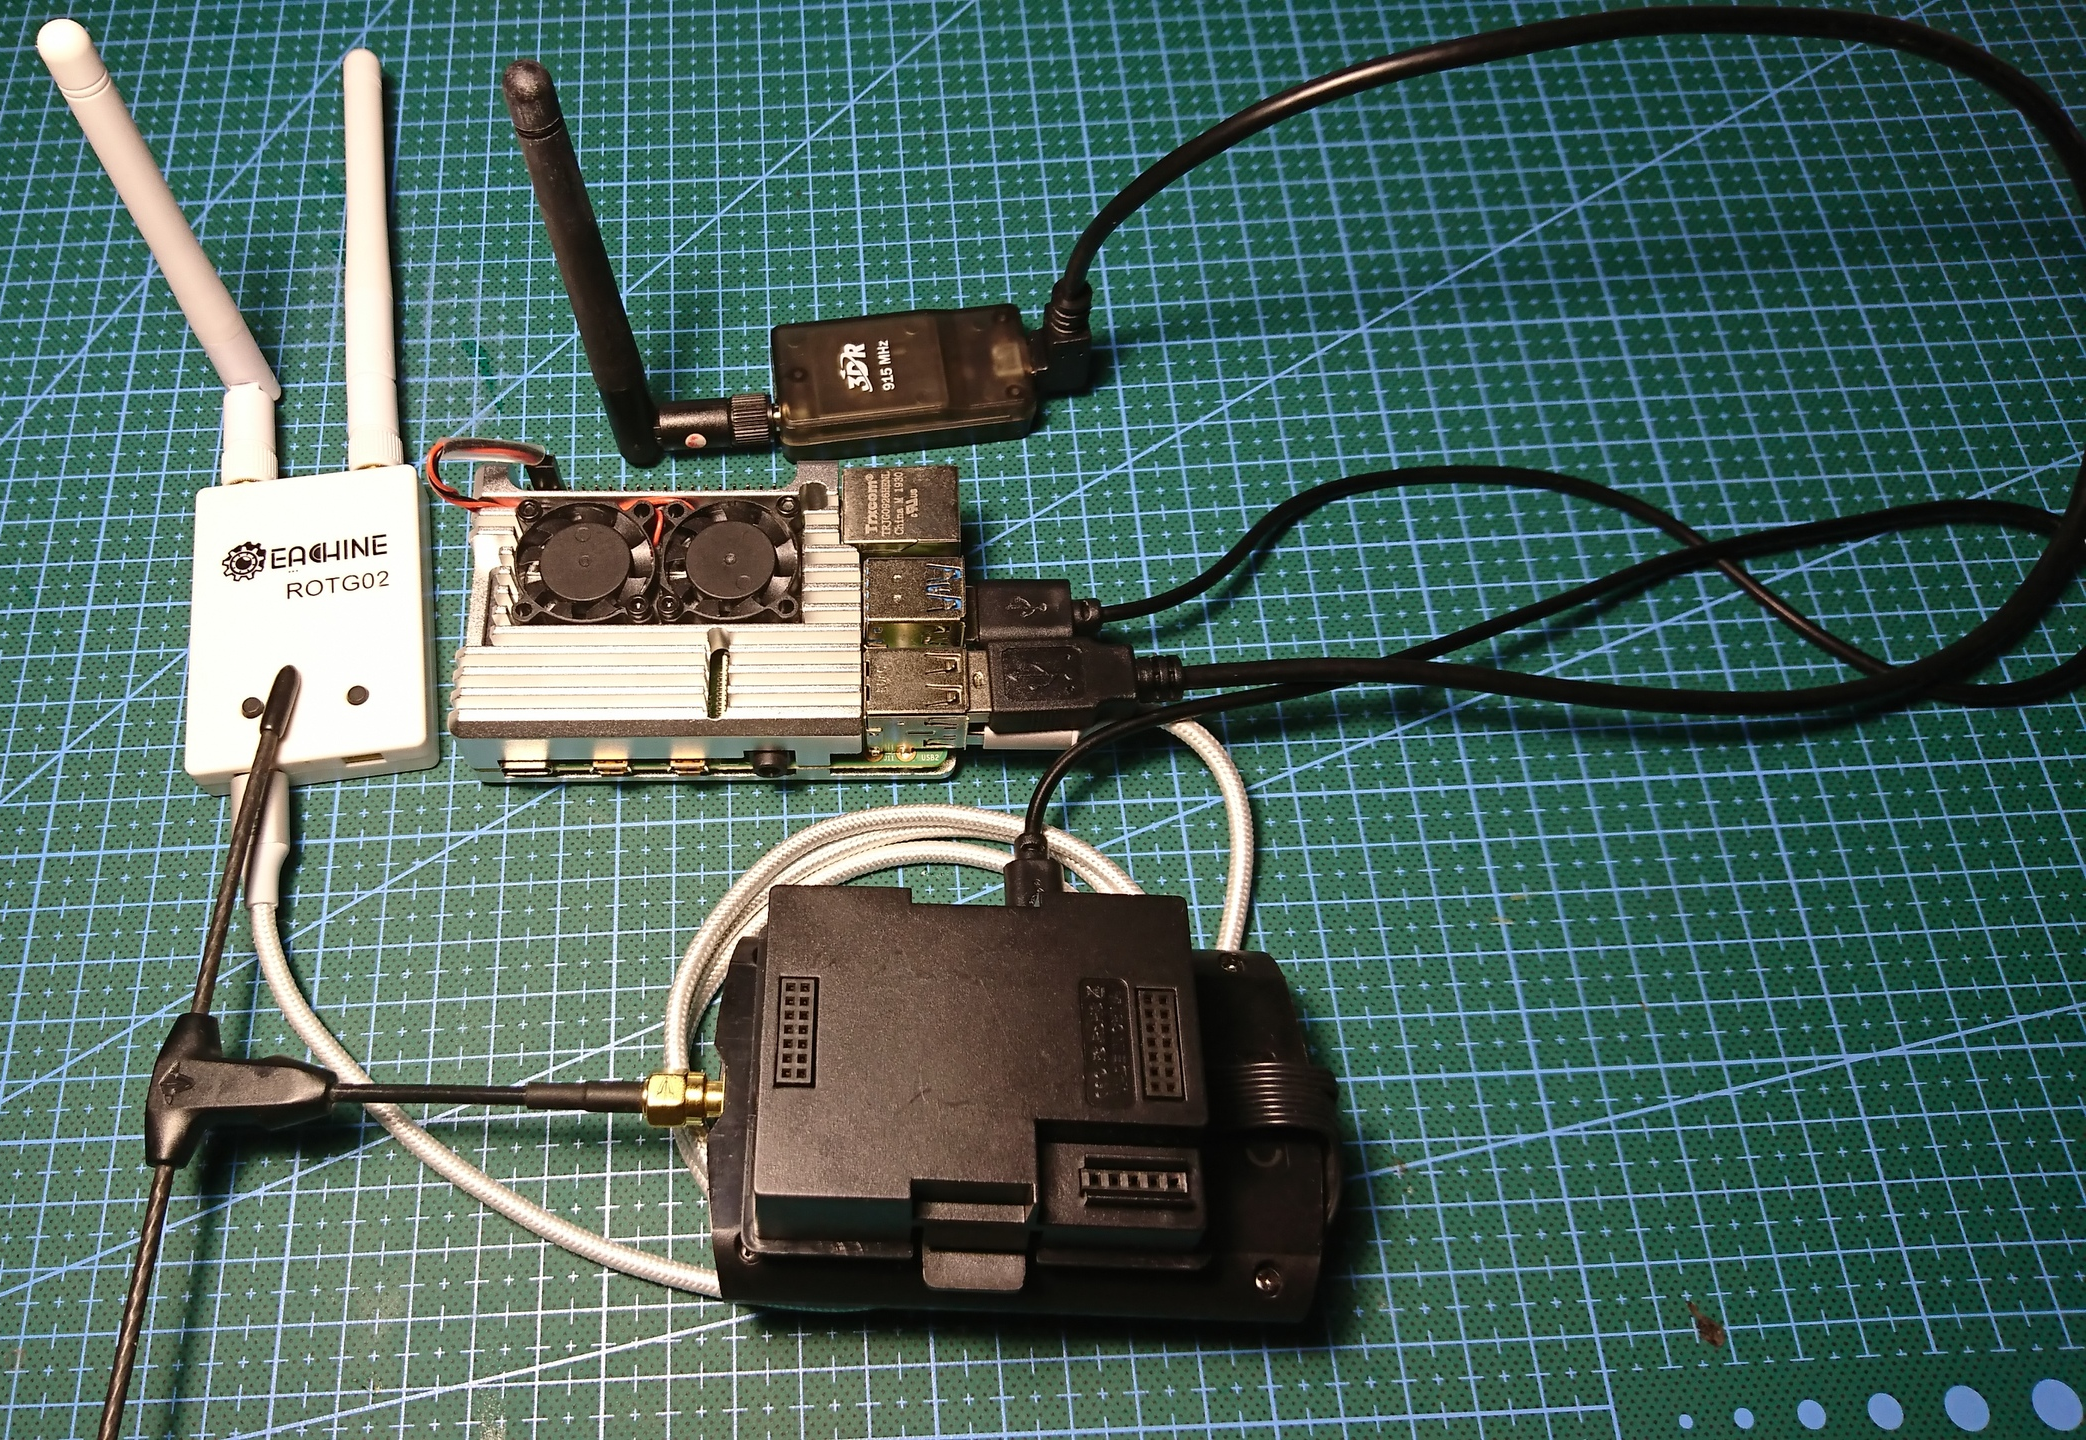
\includegraphics[width=0.5\linewidth]{./pics/qgc}
	\caption{Первый экспериментальный образец наземной станции
	}
	\label{fig:ns} % эта метка позволяет ссылаться на рисунок в тексте
\end{figure}

Однако в ходе выполнения научно-исследовательской работы \cite{nir3} был выявлен более оптимальный способ обмена информации -- по wifi-соединению. Такой способ позволяет уменьшить задержку, количество компонентов, а значит и стоимость комплекта, и использовать персональный компьютер в качестве наземной станции. 
 % дописать преимущества такого решения
%куда необходимо поставить несколько программных решений и настроить взаимодействие между ними.

Таким образом, наземная станция представляет собой компьютер, находящийся в одной подсети с RPi дрона.
ПО наземной станции представляет собой совокупность таких решений как:
\begin{itemize}
	\item операционная система семейства ubuntu версии 16 / 18 на базе ядра linux версии 5.3.0*;
	\item пакетов ros-*;
	\item mavros;
	\item gstreamer;
	\item aruco\_gridboard в связке с gscam.
\end{itemize}
%дописать как это работает. у меня теперь малина регистрирует изображение с камеры, передает на наземную станцию..

\subsection{Конфигурация наземной станции}

\subsubsection{Настройка MAVROS}

Первым делом производится запуск ROS среды посредством roscore. Далее настраиваются конфигурационные файлы.

Для получения телеметрии полетного контроллера необходимо в файле /opt/ros/melodic/share/mavros/launch/px4.launch поменять параметр fcu\_url, указав нужный адрес и порт. Параметр gcs\_url задает адрес для проксирования MAVLink сообщений под нужды qgroundcontrol (листинг \ref{lst:9}):
\begin{Program}[H]
	\caption{Измененные параметры в launch файле mavros} \label{lst:9}
	\begin{MyCode}
	<arg name="fcu_url" default="tcp://192.168.1.148:2000?ids=1,240"/>   
	<arg name="gcs_url" default="udp://@127.0.0.1:14555"/>
	\end{MyCode}
\end{Program}

\subsubsection{Подготовка инструментов для получения и обработки видеопотока}
Для получения трансляции и публикации топиков с изображением с камеры используется пакет gscam. Он собирается из репозитория \url{https://github.com/ros-drivers/gscam} командами, представленными в листинге \ref{lst:10}:
\begin{Program}[H]
	\caption{Сборка gscam} \label{lst:10}
	\begin{MyCode}
	$ git clone https://github.com/ros-drivers/gscam
	$ cd gscam
	$ cmake -DGSTREAMER_VERSION_1_x=On
	$ сmake install
	\end{MyCode}
\end{Program}

Распознавание карты aruco маркеров на изображении, получаемом из топиков gscam, и публикацию полученных координат в топик /vision/pose производит пакет aruco\_gridboard. Команды для сборки этого пакета представлены в листинге \ref{lst:11}:
\begin{Program}[H]
	\caption{Сборка aruco\_gridboard} \label{lst:11}
	\begin{MyCode}	
	$ cd ~/catkin_ws/src
	$ git clone https://github.com/anbello/aruco_gridboard.git
	$ cd ..
	$ catkin_make
	$ source devel/setup.bash
	$ catkin_make --only-pkg-with-deps aruco_gridboard
	\end{MyCode}
\end{Program}

Проделанных шагов достаточно, чтобы на наземной станции отобразить положение дрона относительно карты маркеров.
  % третья глава - в файле part3.tex
\pagebreak

\section{Глава 4. Проектирование системы для отправки сообщений на борт дрона с наземной станции}

Отправка видеопотока производится за счет UDP пакетов.  Данный протокол не гарантирует доставку сообщений, но позволяет уменьшить задержку получения потока, что более критично. Проверены кодеки jpeg, h264, omxh264enc, из них самым стабильным по задержке оказался h264. Задержка составила 150 мс.

После включения дрона и загрузки ОС RPi производится удаленное подключение к Raspberry Pi.
Запускается gstreamer для передачи изображения с rpicamsrc на адрес наземной станции UDP пакетами. На наземной станции запускается gstreamer для их получения. Команды представлены на листинге \ref{lst:12}:
\begin{Program}[H]
	\caption{Измененные параметры в launch файле mavros} \label{lst:12}
\begin{MyCode}
# На наземной станции запускается:
$ gst-launch-1.0 udpsrc port=5000 ! gdpdepay !\
rtph264depay ! avdec_h264 ! videoconvert !\
autovideosink sync=false
	
# На Raspberry Pi:
$ gst-launch-1.0 rpicamsrc bitrate=1000000 !\
'video/x-h264,width=640,height=480' ! h264parse !\
queue ! rtph264pay config-interval=1 pt=96 ! gdppay !\
udpsink host=[IP ПК] port=5000
	
\end{MyCode}
\end{Program}
\begin{MyCode}
	На ПК запускается:
	\$ gst-launch-1.0 udpsrc port=5000 ! gdpdepay ! rtph264depay ! avdec_h264 ! videoconvert ! autovideosink sync=false
	
	На Raspberry:
	\$ gst-launch-1.0 rpicamsrc bitrate=1000000 ! 'video/x-h264,width=640,height=480' ! h264parse ! queue ! rtph264pay config-interval=1 pt=96 ! gdppay ! udpsink host=[IP ПК] port=5000
	%\$ gst-launch-1.0 -v rpicamsrc bitrate=10000000 rotation=180 exposure-mode=10 awb-mode=0 awb-gain-red=1 awb-gain-blue=2 iso=800 shutter-speed=10000 contrast=50 ! "image/jpeg,width=640,height=480,framerate=30/1" ! udpsink host=192.168.1.148 port=9000
	
\end{MyCode}
%https://www.raspberrypi.org/forums/viewtopic.php?t=196176

%https://docs.opencv.org/master/db/da9/tutorial_aruco_board_detection.html
%https://diydrones.com/group/voltarobots/forum/connect-telemetry-through-tcp-udp?commentId=7447824%3AComment%3A1590641
%https://stackoverflow.com/questions/7669240/webcam-streaming-using-gstreamer-over-udp

%Для использования аппаратного кодирования:
%\begin{MyCode}
%PC(autovideosink sync=false not needed for gscam):
%gst-launch-1.0 udpsrc port=5000 ! gdpdepay ! rtph264depay ! avdec\_h264 ! videoconvert ! autovideosink sync=false

%RPI stream:

%gst-launch-1.0 rpicamsrc bitrate=1000000 ! "video/x-raw,width=640,height=480,framerate=30/1" ! omxh264enc target-bitrate=1000000 control-rate=variable ! 'video/x-h264,width=640,height=480'! h264parse ! queue ! rtph264pay config-interval=1 pt=96 ! gdppay ! udpsink host=192.168.1.253 port=5000
%\end{MyCode}

tab-1 (запуск нод gscam и aruco\_gridboard по полученному топику): 
export GSCAM\_CONFIG="udpsrc port=5000 ! gdpdepay ! rtph264depay ! avdec\_h264 ! videoconvert"
roslaunch aruco\_gridboard detection\_rpicam.launch

tab-2 (запуск окружения маврос): roslaunch mavros apm.launch

tab-3 (The messages SET\_GPS\_GLOBAL\_ORIGIN and a SET\_HOME\_POSITION are sent with a script before starting to use the system.): rosrun aruco\_gridboard set\_origin.py

tab-4 (запуск rviz на усмотрение): rosrun rviz rviz -d catkin\_ws/src/aruco\_gridboard/data/aruco\_grid.rviz

запуск rpi
gst-launch-1.0 rpicamsrc bitrate=1000000 ! 'video/x-h264,width=640,height=480' ! h264parse ! queue ! rtph264pay config-interval=1 pt=96 ! gdppay ! udpsink host=192.168.1.53 port=5000

для задержки в 80мс на пк:\\
clever@clever-dev: gst-launch-1.0 udpsrc port=5000 ! "image/jpeg,width=640,height=480,framerate=30/1" ! jpegdec ! videoconvert ! autovideosink sync=false

на рпи:
gst-launch-1.0 rpicamsrc bitrate=10000000 iso=800 shutter-speed=10000 contrast=50 ! "image/jpeg,width=640,height=480,framerate=30/1" ! udpsink host=192.168.1.53 port=5000

export GSCAM\_CONFIG="udpsrc port=5000 ! "image/jpeg,width=640,height=480,framerate=30/1" ! jpegdec ! videoconvert"
\$ rostopic echo /mavros/vision\_pose/pose

-----
Собрали через каткин драйвер gscam, запустили roscore, осталось изменить лаунч и получить поток.
Для создания топиков необхходимо настроить маврос.

В /opt/ros/melodic/share/mavros/launch/apm.launch меняется параметр fcu\_url для общения с телеметрией по порту полетника с помощью ser2net proxy:
<arg name="fcu\_url" default="tcp://192.168.10.16:2000" />
% ~\ref{fig:px4}
\begin{figure}[H]
	\centering
	\includegraphics[width=0.9\linewidth]{pics/px4}
	\caption{ GStreamer pads (sink, src\_0, src\_1)
	}
	\label{fig:px4}
\end{figure}
  % четвертая глава - в файле part4.tex
\pagebreak

\section{Создание экспериментального образца}
//фотография
//характеристики
//процесс сборки
//проверка работы
//перенести подробности из парт2
\subsection{Выбор компонентов квадрокоптера}
Проведен анализ рынка радиоуправляемых квадрокоптеров и замечено, что готовых вариантов, подходящих для взаимодействия с разрабатываемой наземной станцией, нет. В связи с чем необходимо подобрать компоненты и собрать вручную.

\subsection{Выбор компонентов наземной станции}
\subsection{Сборка}
\subsection{Проверка работы экспериментального образца}
% ~\ref{fig:map}
\begin{figure}[H]
	\centering
	\includegraphics[width=0.5\linewidth]{pics/map}
	\caption{Карта маркеров
	}
	\label{fig:map}
\end{figure}

% ~\ref{fig:aruco_detect}
\begin{figure}[H]
	\centering
	\includegraphics[width=0.5\linewidth]{pics/aruco_detect}
	\caption{Инициализация aruco маркеров
	}
	\label{fig:aruco_detect}
\end{figure}

% ~\ref{fig:time}
\begin{figure}[H]
	\centering
	\includegraphics[width=0.5\linewidth]{pics/time}
	\caption{Время задержки% 0.2с
	}
	\label{fig:time}
\end{figure}
\subsection{smthng}
  % пятая глава - в файле part5.tex
\pagebreak

\section*{\centering ЗАКЛЮЧЕНИЕ}
\addcontentsline{toc}{section}{ЗАКЛЮЧЕНИЕ}
В ходе проведения НИР были выполнены следующие задачи:
\begin{enumerate} 
	\item Изучение предметной области
	\item Разработка архитектуры микродрона
	\item Разработка архитектуры наземной станции
	\item Исследование протоколов общения дрона и наземной станции
	\item Создание экспериментального образца
\end{enumerate}
Спроектированный экспериментальный образец наземной станции и квадрокоптера позволяет разработать программную часть для автономных полетов квадрокоптера.
\pagebreak

\addcontentsline{toc}{section}{СПИСОК ИСПОЛЬЗОВАННОЙ ЛИТЕРАТУРЫ}
% ВАЖНО: для корректного отображения в списке литературы ссылок на англ.языке в bibtex-описание источника следует добавить поле 
% langid = {english}
\printbibliography

\pagebreak

\end{document}          

